\documentclass[bachelor, och, labwork]{shiza}

\usepackage{subfigure}
\usepackage{tikz,pgfplots}
\pgfplotsset{compat=1.5}
\usepackage{float}
\usepackage{pdfpages}

\usepackage{titlesec}
\setcounter{secnumdepth}{4}
\titleformat{\paragraph}
{\normalfont\normalsize}{\theparagraph}{1em}{}
\titlespacing*{\paragraph}
{35.5pt}{3.25ex plus 1ex minus .2ex}{1.5ex plus .2ex}

\titleformat{\paragraph}[block]
{\hspace{1.25cm}\normalfont}
{\theparagraph}{1ex}{}
\titlespacing{\paragraph}
{0cm}{2ex plus 1ex minus .2ex}{.4ex plus.2ex}

% --------------------------------------------------------------------------%


\usepackage[T2A]{fontenc}
\usepackage[utf8]{inputenc}
\usepackage{graphicx}
\graphicspath{ {./images/} }
\usepackage{tempora}

\usepackage[sort,compress]{cite}
\usepackage{amsmath}
\usepackage{amssymb}
\usepackage{amsthm}
\usepackage{fancyvrb}
\usepackage{listings}
\usepackage{listingsutf8}
\usepackage{longtable}
\usepackage{array}
\usepackage[english,russian]{babel}

\usepackage[hidelinks]{hyperref}
\usepackage{url}
\usepackage{multirow}
\usepackage{underscore}
\usepackage{setspace}
\usepackage{indentfirst} 
\usepackage{mathtools}
\usepackage{amsfonts}
\usepackage{enumitem}
\usepackage{tikz}
\usepackage{minted}

\newcommand{\eqdef}{\stackrel {\rm def}{=}}
\newcommand{\specialcell}[2][c]{%
\begin{tabular}[#1]{@{}c@{}}#2\end{tabular}}

\renewcommand\theFancyVerbLine{\small\arabic{FancyVerbLine}}


\begin{document}

\includepdf{tit29.pdf}

%-------------------------------------------------------------------------------

\tableofcontents

\section{Цель работы}
\textbf{Цель работы:}Ознакомление с основными характеристиками логических элементов 
и основами синтеза логических схем.

\section{Задание 1}
Построим схему основных базовых логических элементов:

\begin{figure}[H]
    \centering
    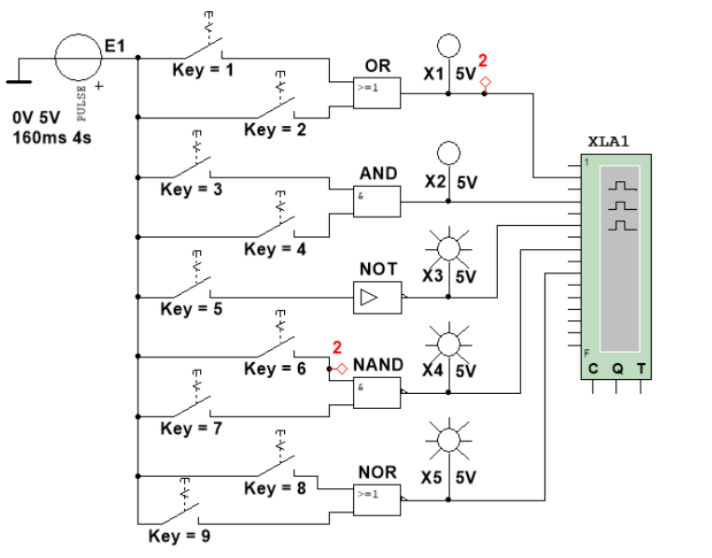
\includegraphics[width=0.8\textwidth]{pic1/1.png}
    \caption{}
\end{figure}

Оперируя ключами $1, 2, ..., 9$ сформируем все возможные комбинации аргументов 
$х_1$ и $х_2$ ($00, 01, 10, 11$) на входе дизъюнктора ($OR$), конъюнктора ($AND$), 
штриха Шеффера (NAND) и стрелки Пирса (NOR) и запишем значения выходных 
логических функций $y_k$ (0 или 1) в таблицу.

\begin{table}[h]
    % \begin{center}
    \centering{
    \begin{tabular}{|lll|lll|ll|lll|lll|}
    \hline
    \multicolumn{3}{|l|}{OR} & \multicolumn{3}{l|}{AND} & \multicolumn{2}{l|}{NOT} & \multicolumn{3}{l|}{NAND} & \multicolumn{3}{l|}{NOR} \\ \hline
    \multicolumn{1}{|c|}{$\text{X}_1$} & \multicolumn{1}{l|}{$\text{X}_2$} & Y & \multicolumn{1}{l|}{$\text{X}_1$} & \multicolumn{1}{l|}{$\text{X}_2$} & Y & \multicolumn{1}{l|}{X} & Y & \multicolumn{1}{l|}{$\text{X}_1$} & \multicolumn{1}{l|}{$\text{X}_2$} & Y & \multicolumn{1}{l|}{$\text{X}_1$} & \multicolumn{1}{l|}{$\text{X}_2$} & Y \\ \hline
    \multicolumn{1}{|l|}{0} & \multicolumn{1}{l|}{0} & 1 & \multicolumn{1}{l|}{0} & \multicolumn{1}{l|}{0} & 0 & \multicolumn{1}{l|}{\multirow{2}{*}{0}} & \multirow{2}{*}{1} & \multicolumn{1}{l|}{0} & \multicolumn{1}{l|}{0} & 1 & \multicolumn{1}{l|}{0} & \multicolumn{1}{l|}{0} & 1 \\ \cline{1-6} \cline{9-14}
    \multicolumn{1}{|l|}{0} & \multicolumn{1}{l|}{1} & 1 & \multicolumn{1}{l|}{0} & \multicolumn{1}{l|}{1} & 0 & \multicolumn{1}{l|}{} & & \multicolumn{1}{l|}{0} & \multicolumn{1}{l|}{1} & 0 & \multicolumn{1}{l|}{0} & \multicolumn{1}{l|}{1} & 1 \\ \hline
    \multicolumn{1}{|l|}{1} & \multicolumn{1}{l|}{0} & 1 & \multicolumn{1}{l|}{1} & \multicolumn{1}{l|}{0} & 0 & \multicolumn{1}{l|}{\multirow{2}{*}{1}} & \multirow{2}{*}{0} & \multicolumn{1}{l|}{1} & \multicolumn{1}{l|}{0} & 0 & \multicolumn{1}{l|}{1} & \multicolumn{1}{l|}{0} & 1 \\ \cline{1-6} \cline{9-14}
    \multicolumn{1}{|l|}{1} & \multicolumn{1}{l|}{1} & 1 & \multicolumn{1}{l|}{1} & \multicolumn{1}{l|}{1} & 1 & \multicolumn{1}{l|}{} & & \multicolumn{1}{l|}{1} & \multicolumn{1}{l|}{1} & 0 & \multicolumn{1}{l|}{1} & \multicolumn{1}{l|}{1} & 0 \\ \hline
    \end{tabular}
    }
    % \end{center}
    
    
    \end{table}



\section{Задание 2}
Соберем схему для реализации заданной логической функции:

\begin{center}$y=(ab+\urcorner c)(\urcorner a+\urcorner b+c)(a+b+c)$\end{center}

\begin{figure}[H]
    \centering
    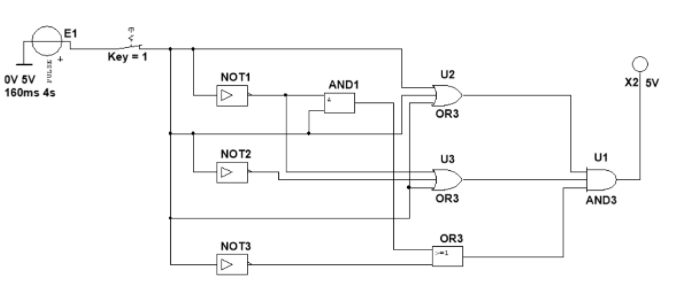
\includegraphics[width=0.8\textwidth]{pic1/2.png}
    \caption{}
\end{figure}

Функция равна нулю при любых входных сигналах

\section{Вывод}
В ходе лабораторной работы мы ознакомились с основными характеристиками логических
элементов, научились строить модели схем в специальном программном обеспечении,
а также, оперируя определенными ключами, перебрали возможные комбинации в
одной из реализации схем, что позволило получить ансамбль выходных данных
для всевозможных вариациях входных значений. Также ознакомились с основами
синтеза логических схем.

\section{Тестовые задания}

\subsection{Задание 1}
    Укажите признаки характеризующие основные логические элементы:
    
    \begin{enumerate}
        \item используя основные логические операции И, ИЛИ и НЕ, можно аналитически
        выразить любую сложную логическую функцию;
        \item минимальный логический базис составляют операции ИЛИ и НЕ или И и НЕ;
        \item входные и выходные сигналы логических элементов могут принимать
        только два значения: логическую 1 и логический 0;
    \end{enumerate}


\subsection{Задание 2}
    Укажите выражение логической функции двух переменных $x_1$ и $x_2$, реализуемой элементом «стрелка Пирса»:
    
    \begin{center}$y = \overline{x_1 + x_2}$\end{center}

\subsection{Задание 3}
     Укажите выражение логической функции двух переменных $x_1$ и $x_2$, реализуемой элементом «штрих Шеффера»:
    
    \begin{center}$y = \overline{x_1x_2}$\end{center}
    
\subsection{Задание 4}
     Укажите выражение логической функции трех переменных $a, b ~\text{и}~ c$, 
     записанной в совершенной дизъюнктивной нормальной форме (СДНФ):

    \begin{center}$y(a, b, c) = \overline{a}bc + a\overline{b}c + ab\overline{c} + abc$\end{center}

\subsection{Задание 5}
    Укажите элемент ИЛИ-НЕ:
    
    \begin{figure}[H]
        \centering    
        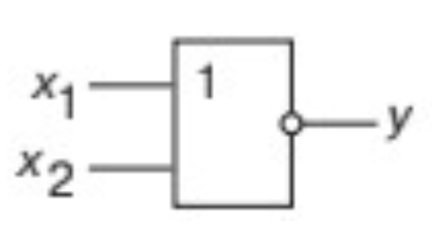
\includegraphics[width=0.4\textwidth]{pic1/3.png}
    \end{figure}

   
\subsection{Задание 6}
    Укажите элемент И:
    
    \begin{figure}[H]
        \centering
        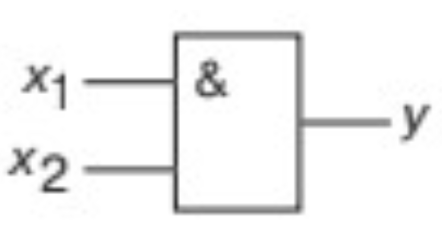
\includegraphics[width=0.4\textwidth]{pic1/4.png}
    \end{figure}

\subsection{Задание 7}
    Укажите значение функции $y = (ab + \overline{c})(\overline{a} + \overline{b})$ если $a = b = c = 1$:
    
    0


\end{document}